\documentclass[aspectratio=169]{beamer}
\usetheme{Madrid}

\usepackage[T2A]{fontenc}
\usepackage[utf8]{inputenc}
\usepackage[russian,english]{babel}
\usepackage{amsmath}
\usepackage{booktabs}
\usepackage{hyperref}
\usepackage{graphicx}

\title{Improving Spatial Reasoning for Pick-and-Place}
\author{Виталий Илюхин, Григорьев Данил}
\date{\today}

\begin{document}

\frame{\titlepage}

\begin{frame}{Постановка задачи}
\begin{itemize}
    \item Цель: повысить качество spatial reasoning в задачах \texttt{pick-and-place} для VLM.
    \item Вход: RGB/RGB-D наблюдения сцены, текстовая инструкция, список объектов-кандидатов.
    \item Выход: корректная пара \texttt{(pick\_object, place\_target)} и успешное физическое выполнение.
    \item Проблема: модели часто понимают объекты, но ошибаются в пространственных отношениях (left/right, nearest/farthest, between, in front of).
\end{itemize}
\end{frame}

\begin{frame}{Почему это актуально}
\begin{columns}[T]
\column{0.52\textwidth}
\begin{itemize}
    \item Пространственные ошибки напрямую приводят к провалам манипуляции и рискам в реальных средах.
    \item Разметка реальных роботических данных дорогая и плохо масштабируется.
    \item Для прикладных сценариев (склад, ассистивная робототехника) важна надежность, а не только ``правильный ответ'' в QA.
    \item Нужен подход, который улучшает рассуждение модели с умеренной стоимостью данных.
\end{itemize}

\column{0.48\textwidth}
\begin{columns}[T,totalwidth=\linewidth]
\column{0.49\linewidth}
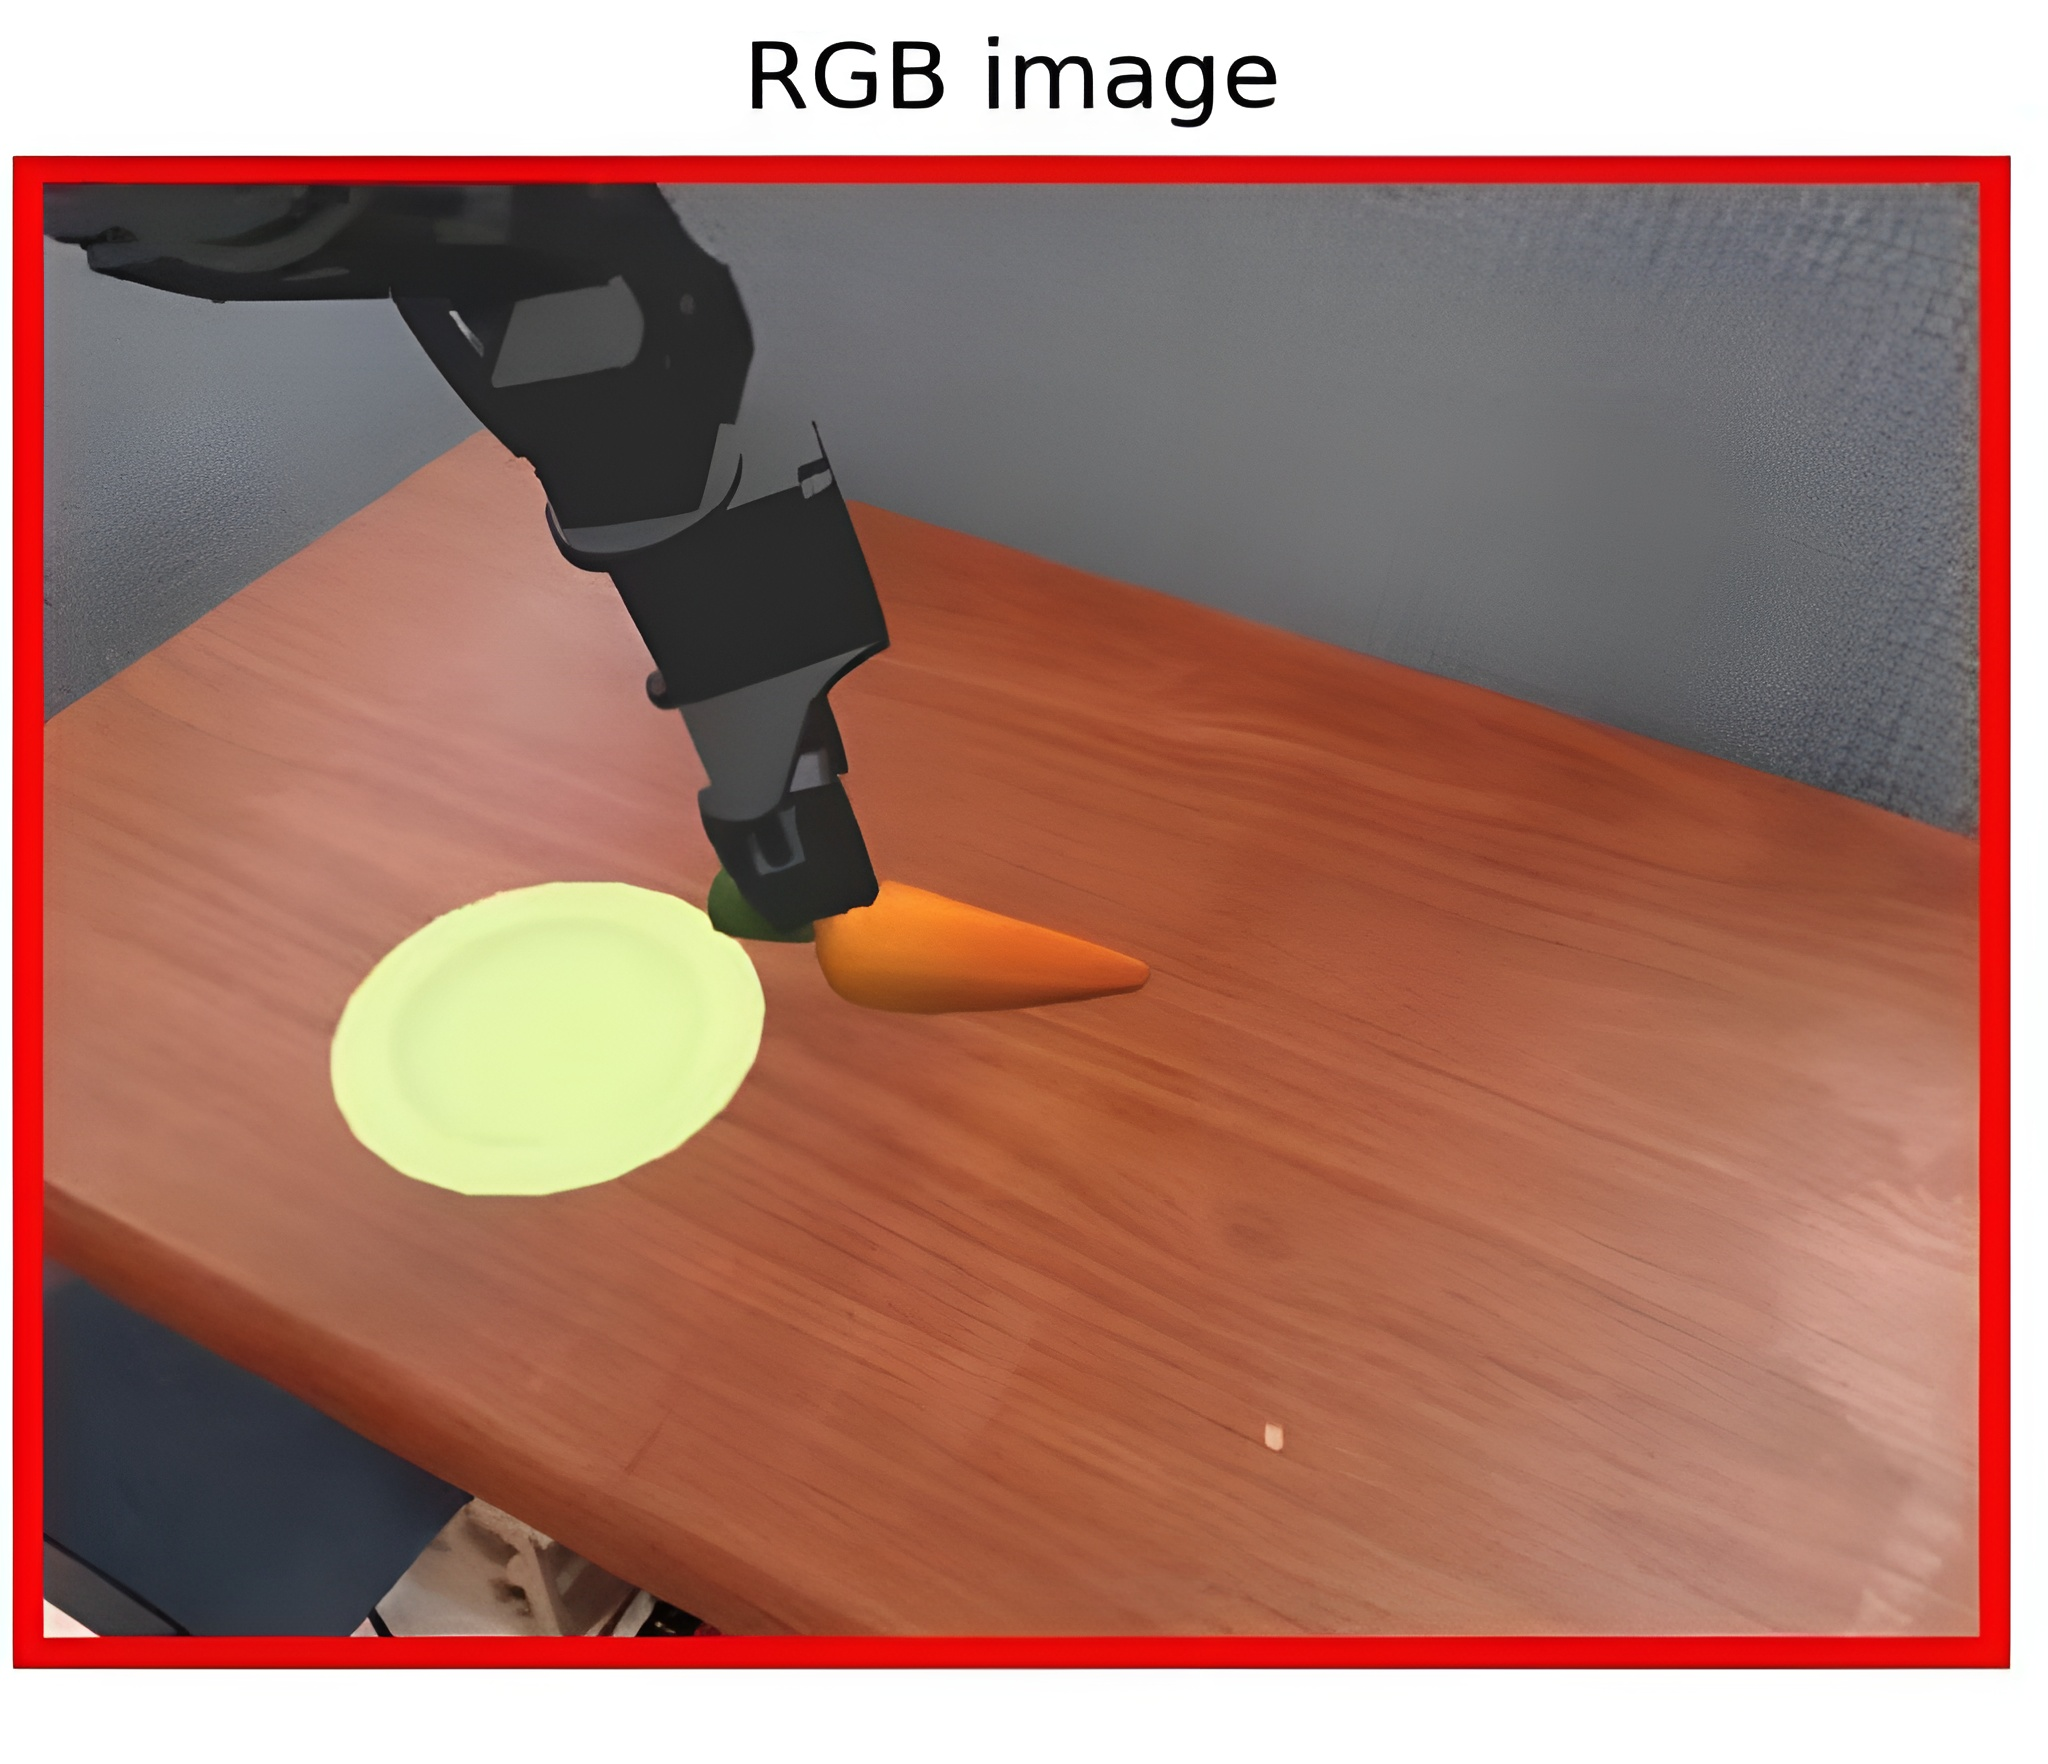
\includegraphics[width=\linewidth]{photo_5397763981511956242_w.jpeg}

\column{0.49\linewidth}
\includegraphics[width=\linewidth]{photo_rgb_sim_2.jpeg}
\end{columns}
\vspace{0.3em}
\scriptsize RGB-наблюдения из симулятора: сложные ракурсы, окклюзии и близкие объекты повышают риск ошибок в spatial reasoning.
\end{columns}
\end{frame}

\begin{frame}{Ключевая идея из статьи}
\begin{itemize}
    \item В \textit{Reasoning Matters for 3D Visual Grounding} показано: \textbf{structured reasoning supervision} важнее, чем просто рост датасета.
    \item Авторы автоматически генерируют 3D сцены и обучающие пары с пошаговым reasoning.
    \item Результат: модель превосходит 3D-GRAND при существенно меньшем объеме обучения (порядка 1.6\% данных).
    \item Вывод для нас: в \texttt{pick-and-place} нужно дообучать VLM не только на ответах, но и на траектории рассуждения.
\end{itemize}
\vspace{0.3em}
\vspace{0.3em}
\footnotesize Ссылка: \href{https://arxiv.org/abs/2601.08811}{arXiv:2601.08811}
\end{frame}

\begin{frame}{Pipeline генерации сцены (для стола)}
\begin{columns}[T]
\column{0.52\textwidth}
\begin{enumerate}
    \item Генерация синтетической \textbf{tabletop}-сцены \texttt{pick-and-place}.
    \item Сэмплирование пространственных шаблонов инструкций.
    \item Построение ``ground truth'' reasoning trace:
    \begin{itemize}
        \item выбор релевантных объектов;
        \item вычисление пространственных признаков/отношений;
        \item выбор финального \texttt{pick} и \texttt{place}.
    \end{itemize}
    \item Дообучение VLM в формате ``instruction $\rightarrow$ reasoning $\rightarrow$ action''.
    \item Валидация на tabletop-сценариях.
\end{enumerate}
\column{0.48\textwidth}
\includegraphics[width=\linewidth]{/home/danil/.cursor/projects/home-danil-Documents-cv-project/assets/image-c02bfd67-2c47-48ab-9536-f95900676624.png}
\end{columns}
\end{frame}

\begin{frame}{Как генерировать данные}
\begin{columns}[T]
\column{0.50\textwidth}
\begin{itemize}
    \item Объекты: категории, размеры, позы, возможные отвлекающие объекты.
    \item Типы отношений:
    \begin{itemize}
        \item бинарные: left/right, in front of/behind, near/far;
        \item составные: between, closest-to-X, farthest-from-Y;
        \item функциональные: ``положи чашку \textit{на} стол справа от ноутбука''.
    \end{itemize}
    \item Вариативность: шум сенсоров, частичная окклюзия, разные ракурсы.
    \item Автофильтрация: отбрасывать двусмысленные и геометрически неконсистентные сцены.
\end{itemize}
\column{0.50\textwidth}
\includegraphics[width=\linewidth]{/home/danil/.cursor/projects/home-danil-Documents-cv-project/assets/image-c02bfd67-2c47-48ab-9536-f95900676624.png}
\vspace{0.2em}
\scriptsize Схема автоматической генерации сцен, парсинга spatial-запросов и построения supervision для дообучения.
\end{columns}
\end{frame}

\begin{frame}{Формат supervision для VLM}
\begin{block}{Training sample}
\small
\textbf{Instruction:} ``Возьми красный куб слева от миски и поставь его за зеленой бутылкой.''\\
\textbf{Reasoning:}
\begin{enumerate}
    \item Найти все ``красные кубы'' и ``миски''.
    \item Проверить отношение ``слева от миски'' для кандидатов.
    \item Для целевого размещения определить область ``за зеленой бутылкой''.
    \item Выбрать финальные \texttt{pick\_id} и \texttt{place\_pose}.
\end{enumerate}
\textbf{Answer:} \texttt{pick\_id=obj\_7, place\_pose=(x,y,z,\theta)}
\end{block}
\end{frame}

\begin{frame}{Обучение}
\begin{itemize}
    \item Базовая модель: VLM/MLLM для vision-language-action.
    \item Режимы:
    \begin{itemize}
        \item SFT на синтетических reasoning-данных;
        \item опционально DPO/RL на успех манипуляции.
    \end{itemize}
    \item Multi-task objective:
\end{itemize}
\[
\mathcal{L} = \lambda_{qa}\mathcal{L}_{qa} + \lambda_{cot}\mathcal{L}_{reason} + \lambda_{act}\mathcal{L}_{action}
\]
\begin{itemize}
    \item \(\mathcal{L}_{qa}\): точность выбора объектов; \(\mathcal{L}_{reason}\): корректность reasoning steps; \(\mathcal{L}_{action}\): точность action-параметров.
\end{itemize}
\end{frame}

\begin{frame}{Оценка: что измеряем}
\begin{block}{1) Task success}
\[
\text{Success Rate} = \frac{\#\text{успешных pick-and-place эпизодов}}{\#\text{всех эпизодов}}
\]
\end{block}

\begin{block}{2) QA / Grounding quality}
\begin{itemize}
    \item \texttt{Pick Accuracy}: верно выбран объект для захвата.
    \item \texttt{Place Accuracy}: верно выбрана зона/поза размещения.
    \item \texttt{Reasoning Consistency}: согласованность reasoning и финального действия.
\end{itemize}
\end{block}

\begin{itemize}
    \item Дополнительно: robust success в OOD-сценах и при визуальном шуме.
\end{itemize}
\end{frame}

\begin{frame}{План экспериментов}
\begin{enumerate}
    \item \textbf{Baseline A}: VLM без reasoning supervision.
    \item \textbf{Baseline B}: VLM с краткими ответами без chain-of-thought.
    \item \textbf{Ours}: VLM с structured reasoning supervision.
\end{enumerate}

\vspace{0.5em}
\begin{table}
\centering
\small
\begin{tabular}{lccc}
\toprule
Метод & Success Rate $\uparrow$ & Pick Acc $\uparrow$ & Place Acc $\uparrow$ \\
\midrule
Baseline A & -- & -- & -- \\
Baseline B & -- & -- & -- \\
Ours & -- & -- & -- \\
\bottomrule
\end{tabular}
\end{table}
\end{frame}

\begin{frame}{Ожидаемый эффект}
\begin{itemize}
    \item Рост \texttt{Success Rate} за счет снижения ошибок в пространственной логике.
    \item Лучшая переносимость на unseen комбинации отношений и объектов.
    \item Меньшая зависимость от дорогой ручной разметки.
    \item Интерпретируемость: reasoning trace помогает диагностировать провалы.
\end{itemize}
\end{frame}

\begin{frame}{Риски и ограничения}
\begin{itemize}
    \item Sim-to-real gap: синтетика не полностью покрывает физику и сенсорные артефакты.
    \item Качество детекции/сегментации ограничивает потолок spatial reasoning.
    \item Возможна ``шаблонность'' reasoning без реального понимания.
\end{itemize}

\vspace{0.5em}
\textbf{Смягчение:}
\begin{itemize}
    \item доменная рандомизация, mixed fine-tuning (synthetic + небольшой real set),
    \item curriculum от простых отношений к compositional инструкциям.
\end{itemize}
\end{frame}

\end{document}
